
\documentclass[10pt,a4paper]{article}
\usepackage[utf8]{inputenc}
\usepackage[french]{babel}
\usepackage[left=2cm,right=2cm,top=2cm,bottom=2cm]{geometry}
\usepackage{hyperref}
\usepackage{amsmath,amssymb}
\usepackage{graphicx}
\usepackage{animate}

%opening
\title{Rapport de Projet}
\author{Nicolas Vadkerti}
\date{}
\usepackage{listings} % Required for inserting code snippets
\usepackage[usenames,dvipsnames]{color} % Required for specifying custom colors and referring to colors by name

\definecolor{DarkGreen}{rgb}{0.0,0.4,0.0} % Comment color
\definecolor{highlight}{RGB}{255,251,204} % Code highlight color

\lstdefinestyle{Style1}{ % Define a style for your code snippet, multiple definitions can be made if, for example, you wish to insert multiple code snippets using different programming languages into one document
language=Perl, % Detects keywords, comments, strings, functions, etc for the language specified
backgroundcolor=\color{highlight}, % Set the background color for the snippet - useful for highlighting
basicstyle=\footnotesize\ttfamily, % The default font size and style of the code
breakatwhitespace=false, % If true, only allows line breaks at white space
breaklines=true, % Automatic line breaking (prevents code from protruding outside the box)
captionpos=b, % Sets the caption position: b for bottom; t for top
commentstyle=\usefont{T1}{pcr}{m}{sl}\color{DarkGreen}, % Style of comments within the code - dark green courier font
deletekeywords={}, % If you want to delete any keywords from the current language separate them by commas
%escapeinside={\%}, % This allows you to escape to LaTeX using the character in the bracket
firstnumber=1, % Line numbers begin at line 1
frame=single, % Frame around the code box, value can be: none, leftline, topline, bottomline, lines, single, shadowbox
frameround=tttt, % Rounds the corners of the frame for the top left, top right, bottom left and bottom right positions
keywordstyle=\color{Blue}\bf, % Functions are bold and blue
morekeywords={}, % Add any functions no included by default here separated by commas
numbers=left, % Location of line numbers, can take the values of: none, left, right
numbersep=10pt, % Distance of line numbers from the code box
numberstyle=\tiny\color{Gray}, % Style used for line numbers
rulecolor=\color{black}, % Frame border color
showstringspaces=false, % Don't put marks in string spaces
showtabs=false, % Display tabs in the code as lines
stepnumber=5, % The step distance between line numbers, i.e. how often will lines be numbered
stringstyle=\color{Purple}, % Strings are purple
tabsize=2
}

\newcommand{\insertcode}[2]{\begin{itemize}\item[]\lstinputlisting[caption=#2,label=#1,style=Style1]{#1}\end{itemize}} 


% \insertcode{"Scripts/example.pl"}{Nena would be proud.} 

\begin{document}

\maketitle


\url{https://github.com/SlaynPool/PROJET_IDO/}
\section*{Sommaire}
\tableofcontents
\setcounter{tocdepth}{2}


\newpage
\vspace*{\stretch{1}}        
\begin{center}

\section*{Introduction}
Mon projet à etait de crée et dévelloper un software OpenSource pour un drone connecté. Mon mémoire à etait fais en collabaration avec Nathan Lys, et vous pourrez trouver dans ce document les parties dont je me suis occupé. Ce projet à essentiellement etait porté sur le devellopement du drone et comment faire voler celui-ci tous en pouvant communiquer avec lui. C'est pourquoi ce mémoire sera divisé en deux parties distincts: Fabriquer le drone, et comment communiquer avec le drone pour à la fois le commander ainsi que récolter des données.  Malheuressement, à cause des actualités sanitaires lié au Covid-19, le projet à etait amputé de la quasi-integralité de la partie pratique, du notament à des problemes de sécurité ( Un drone dans un appartement est rarement une bonne idée ). Nous etudiront donc l'utilisation d'un moteur Brushless, aisni que les bases de l'automatique qui nous seront donc utile pour faire voler le drone. Nous verons aussi comment nous pourrons récolter et envoyer des données ainsi que des videos en direct de notre drone.   \\


\end{center}
\vspace*{\stretch{1}}
\newpage

\section{Faire voler notre drone} 
Pour débuter, nous avons cherché à comprendre et maitriser le controle des moteurs Brushless, qui sont les moteurs couraments utilisés dans l'aeromodelisme. L'idée à donc était de comprendre comment utilisé un moteur brushless, de comprendre le fonctionnement d'un "Electronique Speed Control", ESC, et d'etre capable de controler le moteur, via un microcontroleur.
\subsection{Materiel}
\begin{itemize}
 \item Arduino Uno
 \item 4 Afro ESC 20A
 \item 4 Turnigy Multistar 2216-800kv v2
 
\end{itemize}
\subsection{Un moteur brushless}
Les moteurs brushless, ou moteur sans balais, sont des moteurs qui comparée aux moteurs à charbon, offrent de bien meilleurs perfomances, que ce soit en terme de couple, d'évacution thérmique donc moins sensible à la chauffe. De plus, il sont bien plus solide que les moteurs à charbon. Voici le schema d'un moteur brushless : 

\begin{figure}[h!]
\centering
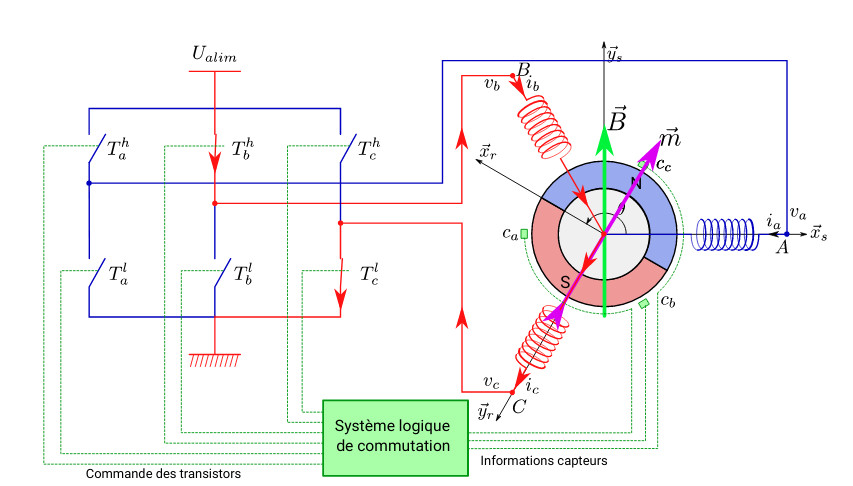
\includegraphics[scale=0.250]{image/1.jpg}
\caption{fonctionnement d'un moteur}
\label{fig:net}
\end{figure}
Le "problème" de ce type de moteur est qu'ils sont difficiles à controler directement. En effet, il faudrait générer trois signals sinusoidales avec des puissances précises ainsi que des déphasages très précis pour exploiter completement le moteur. C'est pour cela que nous allons nous servir d'ESC pour les controler.

\subsection{Les ESC}
 Comme ennoncé précedement, l'ESC aura donc pour objectif de controler notre moteur, et ainsi nous "simplifier" le controle de celui ci. Il existe plusieurs protocoles numeriques pour communniquer avec L'ESC. Cependant, le plus pratique est d'utiliser un signal PWM. Le PWM est la solution la plus pratique car il est très simple de généré un signal PWM grâce à un Arduino.
\subsection{Controle d'un moteur}
Une fois le moteur relié à l'ESC, on peut commencer à controler le moteur, pour les ESC dont on dispose, on utilise la modulation PWM (Modulation à largeur d'impulsion). Durant notre phase de test on a simplement alimenté l'ESC, avec une alimentation réglé sur 14,8V (comme notre batterie). Nous avons ensuite, identifié sur la documentation de l'esc, le pin "SIGNAL", et relié celui ci à un pin de l'arduino capable de généré un PWM (3,5,6,10 et 11). 

Voici le code utilisé pour tester le moteur grâce à la librarie `Servo.h` :
\insertcode{code/1.ino}{Code basique pour controller des moteurs}

 On peut également utiliser la fonction `writeMicroseconds(usec)` afin d'avoir une meilleure préçision pour la puissance utilisé. On va donc avoir de 1060usec à 1430usec pour faire tourner notre moteur. Soit un total de 350 valeurs différentes, à la place de 72 pour la fonction `write`. On va donc utilisé celle-ci sachant qu'elle est plus préçise.

\subsection*{Explication pour la limite du moteur de 12 à 84}
Lorsque l'on "attach" le moteur à un pin, on lui donne 1000us et 2000us. Sur la documentation de l'ESC on nous spécifie 1060us et 1860us. Si on fait un produit en croix entre les valeurs dont on dispose on a :\\

\begin{tabular}{|l|l|}
    Période  & Angle  \tabularnewline    \hline
    1000  & 0  \tabularnewline    \hline
    1060  & 12,6 \tabularnewline    \hline
    1430  & 84,6  \tabularnewline    \hline
    2000  & 180  \tabularnewline    \hline
    
   
        
 \end{tabular}
 \subsection{Test du moteur}
 Pour tester notre Combo ESC/Moteur, nous avons crée un "banc de test". Celui-ci nous a permis d'utiliser le moteur facilement, en sécurité, ainsi que de faire test sur le poid qu'il peut soulever. Nous avons donc dessiner un banc pour tester notre moteur et construit grâce à la découpeuse laser: \\
 \begin{figure}[h!]
\centering
\includegraphics[scale=0.10]{image/2.jpg}
\caption{Banc de Test}
\label{fig:net }
\end{figure}\\
\newpage
\url{https://www.youtube.com/watch?v=S_VZyjie2YE}\\
\\Comme on peut le voir sur la video ci dessus,  nous arrivons à piloter le moteur en variant la vitesse de rotation. Nous avons même pu faire une estimation du poids que celui ci etait capable de soulever à plein puissance. La platforme où est fixer le moteur pèse 500g et le contrepoid 1,50 kg, un seul de nos moteurs peut donc soulever 1kg donc si nous construisons un Quadcoptère nous pourrons theoriquement soulever 4kg.

\newpage 
\subsection{Calcul des vitesses de rotation des 4 moteurs}
Dans cette partie nous allons voir comment nous pouvons calculer la vitesse de rotations des moteurs en fonction des consignes que nous allons donner au drone. Le probleme peut semblait trivial si nous voulons seulement faire monter ou descendre le drone en altitude, on fais varier uniformément la vitesse des quatres moteurs en fonction de ce que l'on veut. Cependant, si l'on veut faire par exemple une translation horizontal cela devient plus compliqué. C'est pourquoi, nous disponsont d'outils mathématiques pour nous aider. Ceci s'appelle les boucles d'asservisements. Il en existe principalement deux types: Les Boucles Ouvertes et les boucles fermées. Nous allons etudier les deux solutions.
Dans cette partie nous allons introduire plusieurs terme relatife au deplacement du drone. Le roll noté $\phi$, le pitch noté $\theta$, le yaw noté  $\psi $, et le throtlle noté $T$. Voici graphiquement à quoi corresponde ces actions :
 \begin{figure}[h!]
\centering
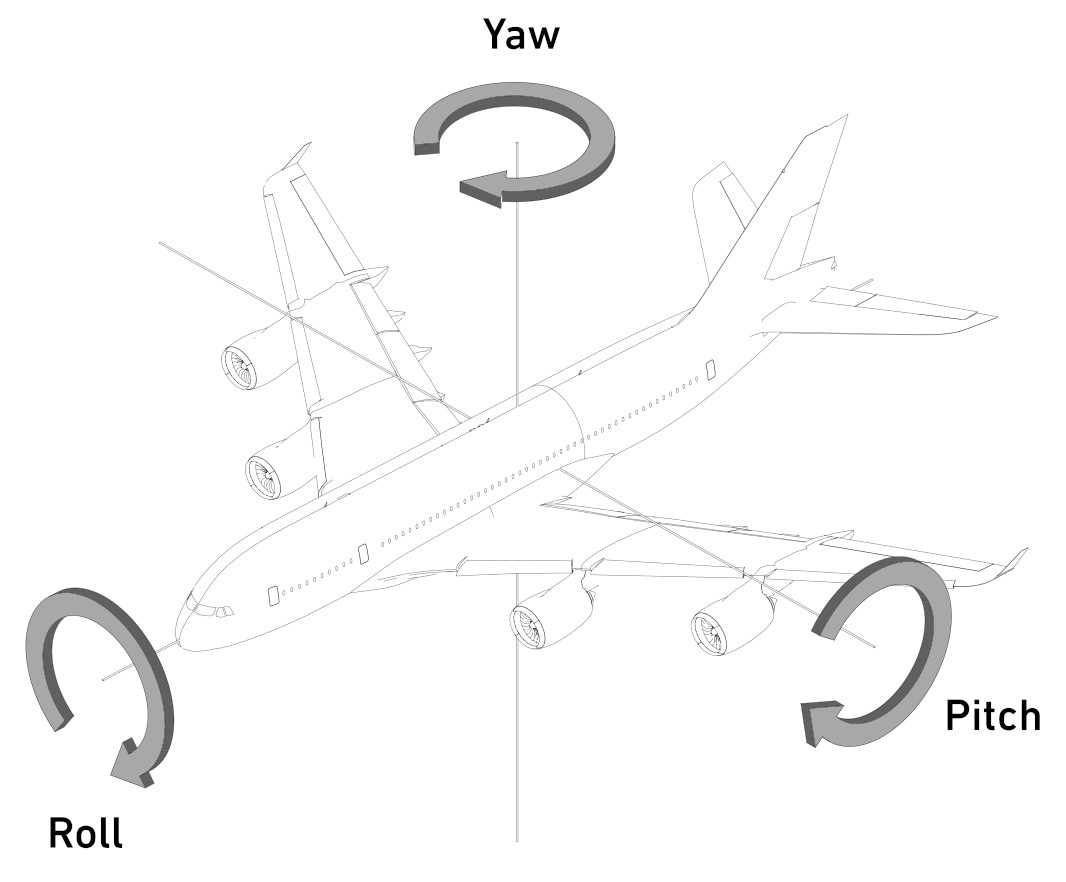
\includegraphics[scale=0.250]{image/yawpitchroll.jpg}
\caption{Illutstration du Yaw Pitch Roll }
\label{fig:net }
\end{figure}\\
Le throtlle correspond à la puissance que l'on va appliquer sur le drone.


\subsection{Systèmes à boucles Ouvertes}
Le principe d'un syteme à boucle ouverte est simple. On va appliquer de facon systematique une action au système sans tenir compte de l'etat actuelle de celui-ci. L'exemple souvant citer et celui-ci: Un arrosoir automatique va arrosser le jardin toute les heures pendant 10 minutes par exemple. Il ne va pas arroser le sol tant que le taux d'humidité ne sera pas correct et arrosera donc meme si il pleut.
Cette solution pourrais fonctionner et ne nesseciterai aucun materiel autre qu'un $\mu$controleur pour faire voler notre drone.
Cependant, cette solution a pour default de ne pas prendre en compte tous les elements qui peuvent interferer avec notre drone, comme le vent ou meme la latence entre le moment ou la consigne est donné et le moment où le moteur est effectivement à la bonne vitesse. Après des recherches, voici comment nous pouvons calculer la vitesse de rotation des moteurs.\\
Source : \url{http://digibuo.uniovi.es/dspace/bitstream/10651/43461/3/TFG_Antu%C3%B1a_Herrero.pdf} page 52
 
 
\begin{equation}\label{xx}
\begin{split}
% \begin{pmatrix}
%  $\phi$\\
%  $\theta$ 
%  
% \end{pmatrix}
\begin{bmatrix}
   \phi \\
   \theta \\
   \psi \\
   T
\end{bmatrix}
=
% \begin{bmatrix}
%  K & -K & -K & K \\
%  K & -K & -K & K 
% \end{bmatrix}
\begin{bmatrix}
    K & -K & -K & K \\
    K & K & -K & -K \\
    K & -K & K & -K \\
    K & K & K & K \\
\end{bmatrix}
 \begin{bmatrix}
    w_1 \\
    w_2 \\
    w_3 \\
    w_4
\end{bmatrix}
\end{split}
\end{equation}

Donc si on veut calculer w1 soit la vitesse de rotation du moteur 1:\\
\begin{equation}\label{xx}
\begin{split}
w_1 =\frac{ \det(\begin{bmatrix}
            \phi & -K & -K & K\\
            \theta & K & -K & -K\\
            \psi & -K & K & -K\\
            T & K & K & K
          \end{bmatrix})}{\det(\begin{bmatrix}
                K & -K & -K & K \\
                K & K & -K & -K \\
                K & -K & K & -K \\
                K & K & K & K \\
          \end{bmatrix})}
\end{split}
\end{equation}
Comme K est une constante, on peut simplifier en:
\begin{equation}\label{xx}
\begin{split}
w_1 =\frac{ \det(\begin{bmatrix}
            \phi & -K & -K & K\\
            \theta & K & -K & -K\\
            \psi & -K & K & -K\\
            T & K & K & K
          \end{bmatrix})}{16 * K}
\end{split}
\end{equation}


Avec cette formule, on peut donc aisement simuler les resultats que l'on pourrais obtenir avec cette methode. J'ai donc programmé en python pour tenter de simuler les resultats: 

  \begin{figure}[h!]
\centering
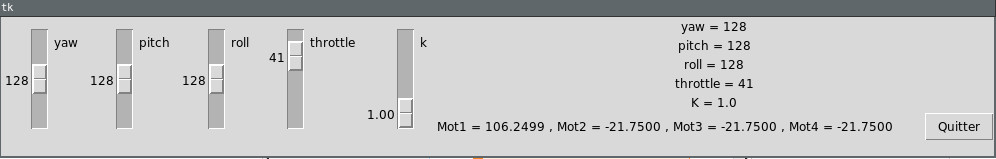
\includegraphics[scale=0.250]{image/SimOpenLoop.jpg}
\caption{Simulation des resultats d'une boucle ouvertes}
\label{fig:net }
\end{figure}
 Comme on peut le voir sur la figure 4, le problème est que je n'arrive pas à simuler des resultats cohérents. En effet, les valeurs entrées sont censé faire monter le drone en altidude seulement, donc que les 4 moteurs aillent les mêmes valeurs appliquées, seulement ce n'est pas le cas. Cette solution est donc éliminer de faite.
 
 \subsection{Le regualteur PID}
 Nous allons maintenant voir le regulateur/Correcteur PID. A l'inverse de la boucle ouverte le régulateur PID est une boucle fermée. L'idée est de mesurer l'etat du système pour pouvoir calculer l'erreur entre ceux que nous voulons et ce que nous avons réellement . Dans notre cas. nous allons mesurer l'inclinaison de notre système. Pour cela, nous pouvons utiliser un accéléromètre comme le MPU6050 très largement utilisé, documenté et fonctionnant grâce au protocole I2C. Voici comment nous pourrions illustrer notre boucle :
   \begin{figure}[h!]
\centering
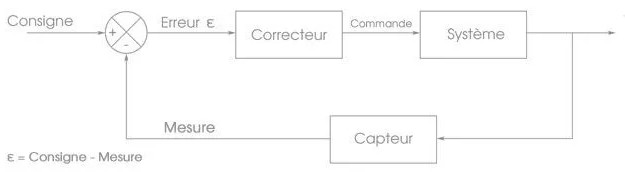
\includegraphics[scale=0.400]{image/SchemaPID.jpg}
\caption{Schema d'une boucle PID}
\label{fig:net }
\end{figure}

Le bloc correcteur va jouer un rôle très important dans notre facon de procéder. En effet, c'est de ce bloc que tire le nom de la méthode. En effet on va succesivement appliquer à l'erreur une action Proportionelle, une Integration dans le temps et une Dérivation et les trois actions seront multiplier par un coefficient que nous pourrons modifier pour améliorer la stabilité du système. Voici comment on exprime mathematiquement ce procéder: \\
\begin{equation}\label{xx}
 u(t) = K_{p}e(t)+K_{i}\int_{0}^{t} e(t') \, \mathrm{d}t'+K_{d}\frac{de(t)}{dt}
\end{equation}
ou :
   \begin{figure}[h!]
\centering
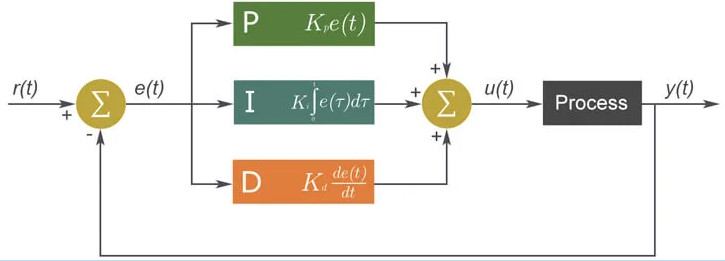
\includegraphics[scale=0.400]{image/IllustrationGrapPID.jpg}
\caption{Un PID}
\label{fig:net }
\end{figure}

\animategraphics[autoplay,loop,width=\textwidth,controls]{5}{image/PID-}{0}{249}
 Si l'animation ne fonctionne pas: \url{https://github.com/SlaynPool/PROJET-IDO/blob/master/Rapport/image/PID.gif}
 \\On peut voir comment on peut ameliorer la stabilité du système en ajustant les coefficients $Kp$, $K_i$ et $K_d$. Cette méthode est très largement utilisé en automatique pour la stabilité quelle apporte, bien quel possède le défault d'être plus lente à calculer dû notamment aux calcules d'intégrales et de dérivées. Cette methode est celle que nous aurions du utiliser si l'on avait pu effectuer la partie pratique du drone. Ainsi nous aurions du procéder comme ceci : 
 \begin{itemize}
  \item Lire l'accelerometre et interpréter les données recu
  \item Lire les consignes recus par la radiocommande par exemple
  \item Calculer l'erreurs entre ce que nous voulons et ce que nous avons
  \item Calculer les valeurs à donner aux ESC pour que les moteurs appliquent la consigne.
  \item Générer les signaux PWM
 \end{itemize}
 Ainsi notre drone serait capable de voler.
\subsection{Conclusion}
Nous avons vu dans cette partie les methodes qu'il faut utiliser pour faire voler notre drone. Cela passe evidement par l'utilisation du Combo ESC/Moteurs que nous utilisons ainsi que la methode pour calculer les consignes à appliquer sur chaques moteurs.

\newpage
\section{Communiquer avec notre drone}
Avant de debuter cette partie, il est important de rappeller brievement le travail effectué par Nathan Lys. En effet, son rôle a etait de mettre en place une liason TCP/IP entre le drône et la base au sol. Il a décider d'utiliser le Wifi, ce qui à pour avantage de nous offrir un debit important, au depit de la portée de communiquation avec notre appareil. Ceci ne pose pas spécialement de soucis car la loi oblige le vol à vue ce qui limite grandement la distance entre la base au sol et le drone. Pour exploiter cet accés Wifi, il a aussi choisi d'utiliser un Raspberry Pi, ce qui signifie que nous aurons deux cartes disctincts sur notre drone. Une avec pour seul but de calculer et controller les moteurs et une autre carte servant à communiquer avec le sol tous types d'informations. Entre le $\mu$controleur et le Raspberry PI nous exploiterons le protocole serie car il est simple a mettre en place via un port USB, permet d'alimenter le $\mu$controleur, et communiquer avec celui-ci. 
\subsection{Quelle sont les elements que nous voulons recevoir et emettre au-(x) drone-(s)}
Comme nous l'avons vu dans la partie précedente, notre drone va avoir besoin de consigne pour voler et etre controlable. De plus, nous voulons implémenter deux caméras sur le drone et donc stream le flux video des deux cameras, et nous aimerions installer une multitude de capteurs sur notre drone. L'utilisation d'un accés Wifi et de faite un reseau IP nous rend très simple la tache. En effet, d'un point de vu pratique, nous n'aurons qu'a ouvrir un socket réseau sur notre Raspberry Pi en ne s'occupant que du contenu des paquets que nous enverrons et que nous recevrons. On peut faire ca dans n'importe quelle language car c'est une operations presque trivial. 




\section*{Documentation/source}
\begin{itemize}
 \item Fonction de la librairie Servo.h :\\
\url{https://www.arduino.cc/en/Reference/Servo}
\item Video du banc de test en activité : \\
\url{https://www.youtube.com/watch?v=S_VZyjie2YE}
\item Moteur : \\
\url{https://cdn-global-hk.hobbyking.com/media/file/288905599X28019X33.pdf}
\item ESC :\\
\url{https://www.flyingtech.co.uk/sites/default/files/product_files/AfroESC\%2020A\%20USER\%20MANUAL\_0.pdf}
\end{itemize}


\end{document}

